% Copyright (C) 2020 Diogo Rodrigues, Breno Pimentel
% Distributed under the terms of the GNU General Public License, version 3

\documentclass[a4paper, 11pt]{report}
\usepackage[top=35mm,bottom=35mm,left=25mm,right=25mm]{geometry} % Margins

% Change section numbers
\renewcommand{\thesection}{\arabic{section}}

% Second page
\usepackage{secondpage}
\usepackage{datetime}

% Appendix
\usepackage{appendix}

% Landscape pages
\usepackage{pdflscape}
\usepackage{multicol}
\setlength\columnsep{50pt}

% Decent underlines
\usepackage[normalem]{ulem}

% Hyper-references
\usepackage{hyperref}

% Imports
\usepackage{import}

% Graphics and images
\usepackage{graphicx} \graphicspath{{./images/}}
\usepackage{tikz}
\usepackage{tikz-qtree}
\usetikzlibrary{automata, positioning, shapes, arrows}
\usepackage[justification=centering,font=small,skip=0.5em]{caption}
\usepackage{subcaption}
\usepackage{float}

\usepackage[binary-units=true]{siunitx} %SI units
\usepackage{pgfplots}
\pgfplotsset{compat=newest} % Allows to place the legend below plot
\usepgfplotslibrary{units} % Allows to enter the units nicely
\sisetup{
  round-mode          = places,
  round-precision     = 2,
}

% Encodings (to render letters with diacritics and special characters)
\usepackage[utf8]{inputenc}
% \DeclareUnicodeCharacter{2192}{\dash}

% Checks and X-marks
\usepackage{xcolor}
\usepackage{pifont}
\definecolor{ForestGreen}{RGB}{34, 139, 34}
\newcommand\greencheckmark{{\color{ForestGreen}\ding{52}}}
\newcommand\redcross{{\color{red}\ding{54}}}

% Language
\usepackage[english]{babel}

% Source code and algorithms
%\usepackage{amsmath}
\usepackage{algorithm}
\usepackage[noend]{algpseudocode}
\usepackage{listings, chngcntr}
\lstset{
	basicstyle=\linespread{0.85}\ttfamily,
	basewidth  = {0.50em,1em},
    frame=tbr, % draw frame at top and bottom of the code
    tabsize=4, % tab space width
    numbers=left, % display line numbers on the left
	showstringspaces=false, % don't mark spaces in strings    
    commentstyle=\color{green}, % comment color
    keywordstyle=\color{blue}, % keyword color
    stringstyle=\color{red}, % string color
    breaklines=true,
    postbreak=\mbox{\textcolor{red}{$\hookrightarrow$}\space}
}
\lstdefinelanguage{cisco}{
    keywords = {
        enable,
        copy, reload,
        configure, terminal, end, interface, switchport, mode,
        access, vlan, show, interfaces, ip, address,
        no, shutdown, exit, nat, inside, outside, route, list, permit,
        pool, source, ovrld, overload, running, id
    },
    morecomment = [l]{\#}
}


% Tables with bold rows
\usepackage{tabularx}
\newcommand\setrow[1]{\gdef\rowmac{#1}#1\ignorespaces}
\newcommand\clearrow{\global\let\rowmac\relax}
\clearrow
\usepackage{multirow}
\usepackage{longtable}

% Tables with vertical center alignment
\usepackage{array}

% Lists and items
\usepackage[inline]{enumitem}

% Math stuff
\usepackage[mathscr]{euscript}
\usepackage{amssymb, latexsym} %Load math symbols like \blacksquare, but also load normal \leadsto arrows
\usepackage{mathtools} % For \text{...}
% \usepackage{enumitem}
% \usepackage{xcolor}
\newcommand{\expnumber}[2]{{#1}\mathrm{e}{#2}} % scientific notation
\newcommand{\degree}{^{\circ}}
\newcommand*\xor{\oplus}
\newcommand\expected[1]{\mathbf{E}[#1]}

% Bibliography
\usepackage{etoolbox}
\makeatletter
\patchcmd{\thebibliography}{%
  \chapter*{\bibname}\@mkboth{\MakeUppercase\bibname}{\MakeUppercase\bibname}}{%
  \section*{Bibliography}}{}{}
\makeatother
\apptocmd{\thebibliography}{\setlength{\itemsep}{2pt}}{}{}
\AtBeginEnvironment{thebibliography}{\small}

% Headers and footers
\usepackage{fancyhdr}
\pagestyle{fancyplain}
\fancyhf{}
\lhead{\fancyplain{}{Configuration of a computer network — Report (RCOM 2020/21)}}
\rhead{\fancyplain{}{Class 2, group 4}}
\lfoot{\fancyplain{}{\leftmark}}
\rfoot{\thepage}

% Email
\newcommand{\email}[1]{
{\texttt{\href{mailto:#1}{#1}} }
}

% Metadata
\title{\Huge Configuration and study of a \\ computer network \\ \vspace*{12pt} \Large Report \\ \vspace*{4pt} \large FEUP - RCOM 2020/21}
\author{
Class 2, group 4 \vspace{0.5em} \\
\begin{tabular}{r l}
	\email{up201800170@fe.up.pt} & Breno Accioly de Barros Pimentel \\
	\email{up201806429@fe.up.pt} & Diogo Miguel Ferreira Rodrigues  \\
\end{tabular}
}
\date{23rd of December, 2020}

% Document
\begin{document}
\maketitle
\begin{secondpage}
    Copyright \copyright 2020--\the\year\ Diogo Rodrigues, Breno Pimentel\par
    \IfFileExists{VERSION}{Version \input{VERSION}}{Draft version}\par
    \immediate\write18{./get-commit-info.sh > COMMIT.tex}
    Built on \today~\currenttime~from \href{https://github.com/dmfrodrigues/feup-rcom-l2}{dmfrodrigues/feup-rcom-l2}, commit \input{COMMIT}\unskip.\par
    Permission is granted to copy and distribute this document under the terms of the
    \href{https://creativecommons.org/licenses/by-nc-nd/4.0/}{Creative Commons Attribution-NonCommercial-NoDerivatives 4.0 International}
    public license.
\end{secondpage}
\clearpage

\pagenumbering{arabic}

\section*{Summary}

This project was elaborated as the second project in the context of the curricular unit Computer Networks (RCOM), part of the Integrated Master in Informatics and Computing Engineering (MIEIC) at the Faculty of Engineering of the University of Porto (FEUP).
It concerns the configuration of a computer network, and its test and study through a developed FTP client.

All objectives were fulfilled, as we successfully implemented in C a simple FTP client for file retrieval over the Internet, and the configured network abided to the guidelines' requirements.

\section*{Introduction} \label{sec:Introduction}

The present project aims at developing a simple FTP client which is to be tested over a configured network.
The source code was developed in the C language, targeting Linux devices.
The goal network is composed of three computers, a switch that implements two virtual sub-networks, and a router to provide Internet access.

This report describes the corresponding project's activities, and is divided into two parts.
In part 1 we address the design, development and testing of the FTP client.
In part 2 we describe the steps on configuring the computer network, over the course of seven short experiments that incrementally contribute to the final network configuration.
This project was tested in the computers of FEUP, room I321, bench 3, with rack computers 2, 3 and 4, a Cisco Catalyst 3560 Series switch and a Cisco 2900 Series router.

\section{Download application} \label{sec:Part1}

A simple FTP client was developed to test the network configuration.

\subsection{Application architecture} \label{sec:Arc}

The application first parses and verifies if the URL abides to \cite{rfc1738} using a regular expression (\texttt{ftp://[<user>:<password>@]<host>/<url-path>}).
Then it finds the IP address with a call to \texttt{gethostbyname} and the application opens a connection using a socket through port 21 to the FTP server. 

After connecting, it logs in to the server, or otherwise logs in as anonymous if no credentials were provided.
Next, it sends a \texttt{PASV} command to the FTP server so it can transfer data in passive mode; if successful, the server will reply
with six bytes, the first four being the server IP address it just opened for transfer, and the other two the port the server is listening on. 

After entering passive mode, the download application opens another socket, using the port provided by the server, where the data will be transferred.
Finally, it copies the file from \texttt{<url-path>} to the current working directory and finishes the connection by sending the \texttt{QUIT} command and closing the sockets.

To build the application, run \texttt{make} in directory \texttt{download}. To test the application, run:

\begin{lstlisting}[frame=none, numbers=none, language=sh]
./download ftp://[<user>:<password>@]<host>/<url-path>
\end{lstlisting}


\subsection{Report of successful download} \label{sec:Dow}

The application was tested in different FTP servers, with files varying in size and type, with and without credentials.
Reports can be found in \ref{listing:6-2-tux33-pipe}, \ref{listing:6-2-tux33-pic2}, \ref{listing:6-5-tux32} and \ref{listing:6-5-tux33}.

\section{Network configuration and analysis} \label{sec:Part2}

\subsection{Experiment 1} \label{sec:Exp1}

\begin{figure}[H]
	\centering
    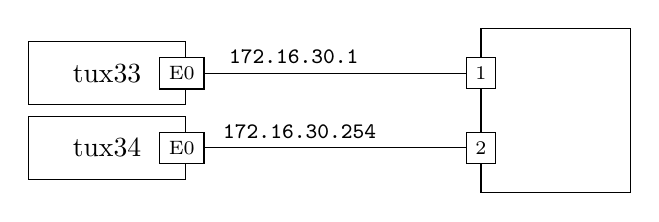
\begin{tikzpicture}[-,>=stealth',node distance=2cm,initial text=$ $,scale=0.95]
        \node at (0,-0) [rectangle,draw,minimum height=0.8cm, minimum width=2cm] (tux33) {tux33};
        \node at (1.0, -0) [rectangle, draw, fill=white] (tux33_E0){ \scriptsize E0 };

        \node at (0,-1.0) [rectangle,draw, minimum height=0.8cm, minimum width=2cm] (tux34) {tux34};
        \node at (1.0, -1) [rectangle, draw, fill=white] (tux34_E0){ \scriptsize E0 };
        


        \draw   (5, +0.6) rectangle ++(2, -2.2);
        \node at (5.0, -0.00) [rectangle, draw, fill=white] (switch_1){ \scriptsize 1 };
        \node at (5.0, -1.00) [rectangle, draw, fill=white] (switch_2){ \scriptsize 2 };

        \draw   (tux33_E0)    edge[above, align=left]     node[xshift=-0.45cm]{\footnotesize \texttt{172.16.30.1  }}          (switch_1)
                (tux34_E0)    edge[above, align=left]     node[xshift=-0.45cm]{\footnotesize \texttt{172.16.30.254}}          (switch_2)
            ;
    \end{tikzpicture}
	\caption{Network architecture for experiment 1}
	\label{fig:network_exp1}
\end{figure}

\noindent
\textbf{Objectives:} connect two computers by configuring their IP addresses.

\subsubsection{Main configuration commands} \label{sec:Com1}

\begin{center}
    \small
    \begin{tabular}{@{}l | m{87mm} | l@{}}
        {\normalfont\textbf{Dev.}} & {\normalfont\textbf{Description}} & {\normalfont\textbf{Commands}}  \\ \hline
        tux33         & Activate \texttt{eth0} interface                     & \begin{lstlisting}[basicstyle=\linespread{0.85}\ttfamily\small, frame=none, numbers=none, language=sh]
ifconfig eth0 up
        \end{lstlisting}               \\
        tux33         & Set \texttt{eth0} IP 172.16.30.1, with 24-bit mask   & \begin{lstlisting}[basicstyle=\linespread{0.85}\ttfamily\small, frame=none, numbers=none, language=sh]
ifconfig eth0 172.16.30.1/24
        \end{lstlisting} \\ \hline
        tux34         & Activate \texttt{eth0} interface                     & \begin{lstlisting}[basicstyle=\linespread{0.85}\ttfamily\small, frame=none, numbers=none, language=sh]
ifconfig eth0 up
        \end{lstlisting}\\
        tux34         & Set \texttt{eth0} IP 172.16.30.254, with 24-bit mask & \begin{lstlisting}[basicstyle=\linespread{0.85}\ttfamily\small, frame=none, numbers=none, language=sh]
ifconfig eth0 172.16.30.254/24
        \end{lstlisting} \\
    \end{tabular}
\end{center}

\subsubsection{Logs analysis} \label{sec:Log1}

IP (Internet Protocol) addresses are a convenient way to refer to interfaces, but to send a frame a device first needs to know the MAC address of the receiving interface.
ARP (Address Resolution Protocol) is used to map an IP address to a MAC address; these mappings are stored in the ARP table, and each device has one such table.
Upon sending a frame, if there is not an entry with the receiver IP in its ARP table, the emitter will broadcast an ARP probe packet with the receiver IP and wait for the corresponding device to announce its presence.

As per log \ref{listing:1-10-tux33.pcapng}, tux33 broadcasts an ARP request in packet \#9 for the desired IP address \texttt{172.16.30.254}.
Then tux34 identifies itself, sending to tux33 another ARP packet with its MAC address \texttt{00:21:5a:5a:7d:74} in packet \#10.

\texttt{ping} generates ICMP (Internet Control Message Protocol) packets. The MAC/IP addresses of the ping packets are the source addresses \texttt{00:21:5a:61:24:92}/\texttt{172.16.30.1} in bytes 0-5
and destination addresses in bytes 6-11 \texttt{00:21:5a:7d:74}/\texttt{172.16.30.254}.

A ARP and IPv4 frames can be identified with the type value 0x806 and 0x800 respectively in the Ethernet II layer.
It is possible to determine if a receiving Ethernet frame have a ICMP layer by checking its IPv4 field and verifying the value 0x01 in the protocol byte.
We could also determine the length of a Ethernet frame by adding the 14 bytes of the Ethernet II layer to the total length described in the IPv4 layer for ICMP packets.
In the case of a ARP packet, the request length is found by adding the Ethernet II layer length and the ARP layer length, the reply length is the previous sum but with a additional padding length. 

The loopback interface allows access to the almost-discontinued Ethernet Configuration Testing Protocol (CTP)\cite{how-ethernet-keepalive-works}\cite[ch.~8]{ethernet}, with provides services similar to \texttt{ping} but on the Data Link layer \cite{jhawk}. It is implemented at least in Cisco routers \cite{jhawk}\cite{whats-a-loop-traffic-in-ethereal} and the switch software configuration guide \cite{cisco-switch-manual} does mention the loopback interface although it does not clearly explain what it is. Due to its specifications, this interface/protocol can serve any of the following purposes:
\begin{enumerate*}[label=(\arabic*)]
    \item \label{itm:connectivity} test connectivity with another station;
    \item \label{itm:loops} check for network loops;
    \item \label{itm:own-issues} check for hardware issues by sending a request to itself \cite{whats-a-loop-traffic-in-ethereal};
    \item \label{itm:self-loop} check for self-looped ports.
\end{enumerate*}
Although CTP was primarily designed for \ref{itm:connectivity} \cite[sec.~8.1]{ethernet}, Cisco now only implements CTP for purposes \ref{itm:own-issues} and \ref{itm:self-loop}\cite{whats-a-loop-traffic-in-ethereal}. In our case it probably serves \ref{itm:self-loop}, as the loopback packets in \ref{listing:1-10-tux33.pcapng} have their source and destination MAC addresses set to those of the device which is consistent with \cite{whats-a-loop-traffic-in-ethereal}. We assume that if the packets were to serve purpose \ref{itm:own-issues} they would not actually be sent down the line, but rather through some internal physical or software medium. As such, computers should just ignore that specific packet, whether or not they implement CTP (if a device does not implement CTP, which is the case for most devices and all mainstream OSs, it will ignore all LOOP requests either way). These packets are sent every 10 seconds.

\subsection{Experiment 2} \label{sec:Exp2}

\begin{figure}[H]
	\centering
    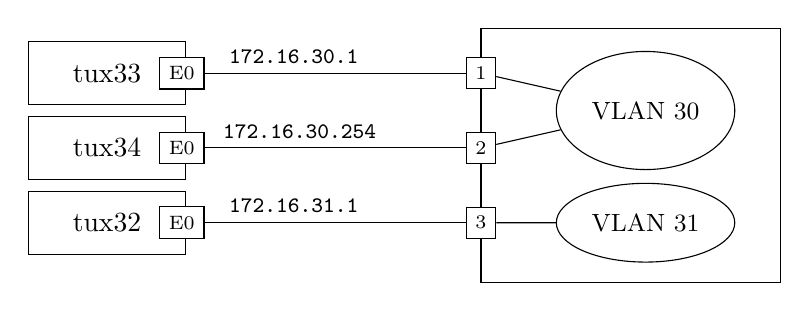
\begin{tikzpicture}[-,>=stealth',node distance=2cm,initial text=$ $,scale=0.95]
        \node at (0,-0) [rectangle,draw,minimum height=0.8cm, minimum width=2cm] (tux33) {tux33};
        \node at (1.0, -0) [rectangle, draw, fill=white] (tux33_E0){ \scriptsize E0 };

        \node at (0,-1.0) [rectangle,draw, minimum height=0.8cm, minimum width=2cm] (tux34) {tux34};
        \node at (1.0, -1) [rectangle, draw, fill=white] (tux34_E0){ \scriptsize E0 };
        
        \node at (0,-2) [rectangle,draw, minimum height=0.8cm, minimum width=2cm] (tux32) {tux32};
        \node at (1.0, -2) [rectangle, draw, fill=white] (tux32_E0){ \scriptsize E0 };

        \draw   (5, +0.6) rectangle ++(4, -3.4);
        \node at (7.2, -0.5) [ellipse, draw, minimum height = 1.5cm, minimum width = 2.0cm, align=center] (VLAN30) {\small VLAN 30};
        \node at (7.2, -2.0) [ellipse, draw, minimum height = 1.0cm, minimum width = 2.0cm, align=center] (VLAN31) {\small VLAN 31};
        \node at (5.0, -0.00) [rectangle, draw, fill=white] (switch_1){ \scriptsize 1 };
        \node at (5.0, -1.00) [rectangle, draw, fill=white] (switch_2){ \scriptsize 2 };
        \node at (5.0, -2.00) [rectangle, draw, fill=white] (switch_3){ \scriptsize 3 };

        \draw   (tux33_E0)    edge[above, align=left]     node[xshift=-0.45cm]{\footnotesize \texttt{172.16.30.1  }}          (switch_1)
                (tux34_E0)    edge[above, align=left]     node[xshift=-0.45cm]{\footnotesize \texttt{172.16.30.254}}          (switch_2)
                (tux32_E0)    edge[above, align=left]     node[xshift=-0.45cm]{\footnotesize \texttt{172.16.31.1  }}          (switch_3)
                
                (switch_1) edge[] (VLAN30)
                (switch_2) edge[] (VLAN30)
                (switch_3) edge[] (VLAN31)
            ;

    \end{tikzpicture}
	\caption{Network architecture for experiment 2}
	\label{fig:network_exp2}
\end{figure}

\noindent
\textbf{Objectives:} implement two virtual LANs in a switch.

\subsubsection{Main configuration commands} \label{sec:Com2}

\begin{center}
    \small
    \begin{tabular}{@{}l | m{93mm} | l@{}}
        {\normalfont\textbf{Dev.}} & {\normalfont\textbf{Description}} & {\normalfont\textbf{Commands}}  \\ \hline
        switch        & Create virtual LAN 30                                 &
            \begin{lstlisting}[basicstyle=\linespread{0.85}\ttfamily\small, frame=none, numbers=none, language=cisco]
configure terminal
vlan 30
end
            \end{lstlisting} \\
        switch        & Assign port 1 to VLAN 30                              & 
            \begin{lstlisting}[basicstyle=\linespread{0.85}\ttfamily\small, frame=none, numbers=none, language=cisco]
configure terminal
interface fastethernet 0/1
switchport mode access
switchport access vlan 30
end
            \end{lstlisting} \\
    \end{tabular}
\end{center}

\subsubsection{Logs analysis} \label{sec:Log2}

To configure VLAN30, we had to create it in the switch, and then add switch port 1 (tux33-E0) and switch port 2 (tux34-E0) to that VLAN.

From log \ref{listing:2-5-tux33.pcapng} we infer tux33 can ping tux34 but cannot ping tux32 (the failed pings to tux32 are not in the log, but we have experimentally verified this outcome from \texttt{ping} output).
From logs \ref{listing:2-7-tux32.pcapng}, \ref{listing:2-7-tux33.pcapng} and \ref{listing:2-7-tux34.pcapng} we see that a broadcast from tux33 can reach tux33 and tux34, but not tux32.
From logs \ref{listing:2-10-tux32.pcapng}, \ref{listing:2-10-tux33.pcapng} and \ref{listing:2-10-tux34.pcapng} we see that a broadcast from tux32 can only reach tux32.
This leads us to conclude there are two virtual networks, VLAN30 which includes tux33 and tux34, and VLAN31 which includes tux32, as well as that there are two different broadcast domains, one for each subnet: \texttt{172.16.31.255} and \texttt{172.16.30.255}.

Upon close inspection of logs \ref{listing:2-7-tux33.pcapng} and \ref{listing:2-7-tux34.pcapng}, it can be seen that the destination of the broadcast issued from tux33 is \texttt{172.16.30.0}.
We tried to analyse this issue, and concluded the most likely option is that we issued the broadcast from tux33 to the wrong IP address (\texttt{172.16.30.0} instead of the obvious broadcast address \texttt{172.16.30.255} for VLAN30), but that somehow the ping was still considered a broadcast as it is also obvious this ping reached tux34.
There are some \cite{ping-subnet-address-1}\cite{ping-subnet-address-2} who mention that historically some devices treat the subnet IP address as a broadcast address.

On inspecting the ping requests, both broadcasts sent from tux33 and tux32 are Ethernet II frames have their destination set to the MAC broadcast address \texttt{ff:ff:ff:ff:ff:ff}, and only the contained IPv4 destination addresses differ.
The switch works on the Data Link layer so it can only understand the Ethernet II frames, not the contained IPv4 packet so it broadcasts both pings in exactly the same way, each in its own subnetwork; so apparently, somewhere in the process of converting the destination IP address to a MAC address, tux33 interpreted \texttt{172.16.30.0} as a broadcast address and framed the IPv4 packet in a frame destined to the MAC broadcast address \texttt{ff:ff:ff:ff:ff:ff}. This is further reinforced by the fact even the \texttt{ping} command recognizes a network address as a broadcast address, assumed from its output \texttt{ping: Do you want to ping broadcast? Then -b. If not, check your local firewall rules} when you try to ping a network IP address without using the \texttt{-b} (broadcast) flag. 

\subsection{Experiment 3} \label{sec:Exp3}

\begin{figure}[H]
	\centering
    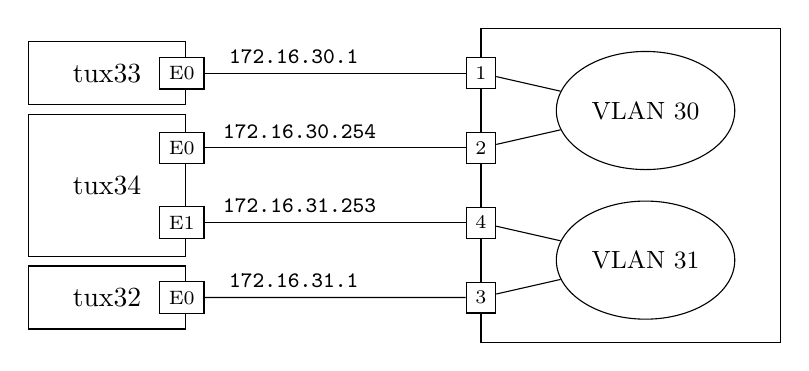
\begin{tikzpicture}[-,>=stealth',node distance=2cm,initial text=$ $,scale=0.95]
        \node at (0,-0) [rectangle,draw,minimum height=0.8cm, minimum width=2cm] (tux33) {tux33};
        \node at (1.0, -0) [rectangle, draw, fill=white] (tux33_E0){ \scriptsize E0 };

        \node at (0,-1.5) [rectangle,draw, minimum height=1.8cm, minimum width=2cm] (tux34) {tux34};
        \node at (1.0, -1) [rectangle, draw, fill=white] (tux34_E0){ \scriptsize E0 };
        \node at (1.0, -2) [rectangle, draw, fill=white] (tux34_E1){ \scriptsize E1 };
        
        \node at (0,-3) [rectangle,draw, minimum height=0.8cm, minimum width=2cm] (tux32) {tux32};
        \node at (1.0, -3) [rectangle, draw, fill=white] (tux32_E0){ \scriptsize E0 };

        \draw   (5, +0.6) rectangle ++(4, -4.2);
        \node at (7.2, -0.5) [ellipse, draw, minimum height = 1.5cm, minimum width = 2.0cm, align=center] (VLAN30) {\small VLAN 30};
        \node at (7.2, -2.5) [ellipse, draw, minimum height = 1.5cm, minimum width = 2.0cm, align=center] (VLAN31) {\small VLAN 31};
        \node at (5.0, -0.00) [rectangle, draw, fill=white] (switch_1){ \scriptsize 1 };
        \node at (5.0, -1.00) [rectangle, draw, fill=white] (switch_2){ \scriptsize 2 };
        \node at (5.0, -2.00) [rectangle, draw, fill=white] (switch_4){ \scriptsize 4 };
        \node at (5.0, -3.00) [rectangle, draw, fill=white] (switch_3){ \scriptsize 3 };

        \draw   (tux33_E0)    edge[above, align=left]     node[xshift=-0.45cm]{\footnotesize \texttt{172.16.30.1  }}          (switch_1)
                (tux34_E0)    edge[above, align=left]     node[xshift=-0.45cm]{\footnotesize \texttt{172.16.30.254}}          (switch_2)
                (tux32_E0)    edge[above, align=left]     node[xshift=-0.45cm]{\footnotesize \texttt{172.16.31.1  }}          (switch_3)
                (tux34_E1)    edge[above, align=left]     node[xshift=-0.45cm]{\footnotesize \texttt{172.16.31.253}}          (switch_4)

                (switch_1) edge[] (VLAN30)
                (switch_2) edge[] (VLAN30)
                (switch_3) edge[] (VLAN31)
                (switch_4) edge[] (VLAN31)
            ;

    \end{tikzpicture}
	\caption{Network architecture for experiment 3}
	\label{fig:network_exp3}
\end{figure}

\textbf{Objectives:} configure a router in Linux.

\subsubsection{Main configuration commands} \label{sec:Com3}

\begin{center}
    \small
    \begin{tabular}{@{}l | m{56mm} | l@{}}
        {\normalfont\textbf{Dev.}} & {\normalfont\textbf{Description}} & {\normalfont\textbf{Commands}}  \\ \hline
        tux34         & Configure tux34-E1 &
            \begin{lstlisting}[basicstyle=\linespread{0.85}\ttfamily\small, frame=none, numbers=none, language=sh]
ifconfig eth1 up
ifconfig eth1 172.16.31.253/24
            \end{lstlisting} \\
        tux34         & Enable IP forwarding & 
        \begin{lstlisting}[basicstyle=\linespread{0.85}\ttfamily\small, frame=none, numbers=none, language=sh]
echo 1 > /proc/sys/net/ipv4/ip_forward
        \end{lstlisting} \\
        tux34         & Disable ICMP echo-ignore-broadcast &  
        \begin{lstlisting}[basicstyle=\linespread{0.85}\ttfamily\small, frame=none, numbers=none, language=sh, escapeinside={(*}{*)}]
echo 0 > /proc/sys/net/ipv4/
    (*\mbox{\textcolor{red}{$\hookrightarrow$}\space}*)icmp_echo_ignore_broadcasts
        \end{lstlisting} \\ \hline
        tux32         & Add route to VLAN30 &  
        \begin{lstlisting}[basicstyle=\linespread{0.85}\ttfamily\small, frame=none, numbers=none, language=sh]
route add -net 172.16.30.0/24 gw 172.16.31.253
        \end{lstlisting} \\ \hline
        tux33         & Add route to VLAN31 &  
        \begin{lstlisting}[basicstyle=\linespread{0.85}\ttfamily\small, frame=none, numbers=none, language=sh]
route add -net 172.16.31.0/24 gw 172.16.30.254
        \end{lstlisting} \\ \hline
        switch        & Add port 4 to VLAN 31 & 
        \begin{lstlisting}[basicstyle=\linespread{0.85}\ttfamily\small, frame=none, numbers=none, language=cisco]
configure terminal
interface fastethernet 0/4
switchport mode access
switchport access vlan 31
end
        \end{lstlisting}
    \end{tabular}
\end{center}

\subsubsection{Logs analysis} \label{sec:Log3}

\begin{center}
    \small
    \begin{tabular}{l | l}
        \textbf{Dev.} & \begin{lstlisting}[basicstyle=\linespread{0.85}\ttfamily\footnotesize, frame=, numbers=none]
Destination     Gateway         Genmask         Flags Metric Ref    Use Iface
            \end{lstlisting} \\ \hline
        tux32 & \lstinputlisting[basicstyle=\linespread{0.85}\ttfamily\footnotesize, frame=, numbers=none, firstline=3]{../../part2/exp3/3-4-tux32.route.txt} \\ \hline
        tux33 & \lstinputlisting[basicstyle=\linespread{0.85}\ttfamily\footnotesize, frame=, numbers=none, firstline=3]{../../part2/exp3/3-4-tux33.route.txt} \\ \hline
        tux34 & \lstinputlisting[basicstyle=\linespread{0.85}\ttfamily\footnotesize, frame=, numbers=none, firstline=3]{../../part2/exp3/3-4-tux34.route.txt}
    \end{tabular}
\end{center}

A forwarding table entry contains the destination IP address, a gateway IP address where data will be sent for routing to the destination IP address, netmask, route flags (the most important flags are \texttt{U} - up and \texttt{G} - gateway), a metric used to choose the fastest route and representing the number of hops to the target, number of references to the route (not used by the Linux kernel), count of route lookups and the interface to which packets will be sent \cite{man-route}.

Each tux has two \textit{routes}, one for VLAN30 and another for VLAN31.
In the case of the routes from tux32 to VLAN31, tux33 to VLAN30 and tux34 to both VLANs, the gateway is set to \texttt{0.0.0.0}; in this context it means the gateway to reach that subnetwork is unspecified, which usually means no intermediate hops are necessary as the system is directly connected to that destination (i.e., the device belongs to said subnetwork), and as such packets will be directly sent to the destination \cite{routing-basics}.
As for the route from tux32 to VLAN31, the IP address of the tux34 interface in VLAN30 is specified as the gateway to access VLAN31, as a request sent to \texttt{172.16.31.253} and directed at an IP address in VLAN30 will be routed by tux34 through \texttt{172.16.30.254}; the route from tux33 to VLAN30 works in the same way. 

ARP tables are all initially empty.
tux33 knows requests to VLAN31 must be made through gateway \texttt{172.16.30.254} (tux33-eth0), but it does not know which MAC address is associated to that IP address.
Thus, in logs \ref{listing:3-8-tux34-eth0.pcapng} and \ref{listing:3-8-tux34-eth1.pcapng}, we see that tux33 broadcasts an ARP request asking for the MAC address of \texttt{172.16.30.254} (tux33-eth0), to which tux34 answers with \texttt{00:21:5a:5a:7d:74}.
By the time tux34 receives its first ping from tux33 to \texttt{172.16.31.1} (tux32-eth0), it does not yet know the MAC address to forward the request to, so because tux34 knows eth1 is connected to VLAN31 it broadcasts an ARP request from \texttt{172.16.31.253} (tux34-eth1) asking for \texttt{172.16.31.1}, to which tux32 answers with its MAC address.

In the same logs, we can see that the ICMP packets being transmitted are ping requests and replies. For each ping sent from tux32, the following sequence of communications is observed:
tux33 sends to \texttt{00:21:5a:5a:7d:74} (tux34-eth0) the ping request to \texttt{172.16.31.1} (tux32-eth0), as tux33 already knows the MAC address for tux34-eth0 and it also knows that requests to VLAN31 must use tux34-eth0 as gateway;
tux34 forwards the ping to \texttt{00:21:5a:61:30:63} (tux32-eth0), its final destination;
tux32 replies to IP address \texttt{172.16.30.1} (\texttt{tux33-eth0}) but sending the reply to MAC address \texttt{00:c0:df:25:26:0a} (\texttt{tux34-eth1}) because this is the MAC address the request came from;
tux34 subsequently forwards the response to \texttt{00:21:5a:5a:7d:74} (tux33-eth0), its final destination.

This means computers tux32 and tux33 build their ARP tables only when they are requested to communicate with the corresponding IP addresses, by means of ARP broadcasts and replies. Additionally, packets carry the final IP addresses they should be sent to, but the frames they are contained in bear the MAC addresses of the immediate destination; this is because IP addresses are used by routers which work with the Network layer and use them to route requests between networks, but frames are managed by the switch which works with the Data Link layer and must be transmitted to MAC addresses within the same network. Thus, the switch only understands what frames are, and tux34 is the responsible for understanding to which network it should route the contained IPv4 request as it acts as a router.

\subsection{Experiment 4} \label{sec:Exp4}

\begin{figure}[H]
	\centering
    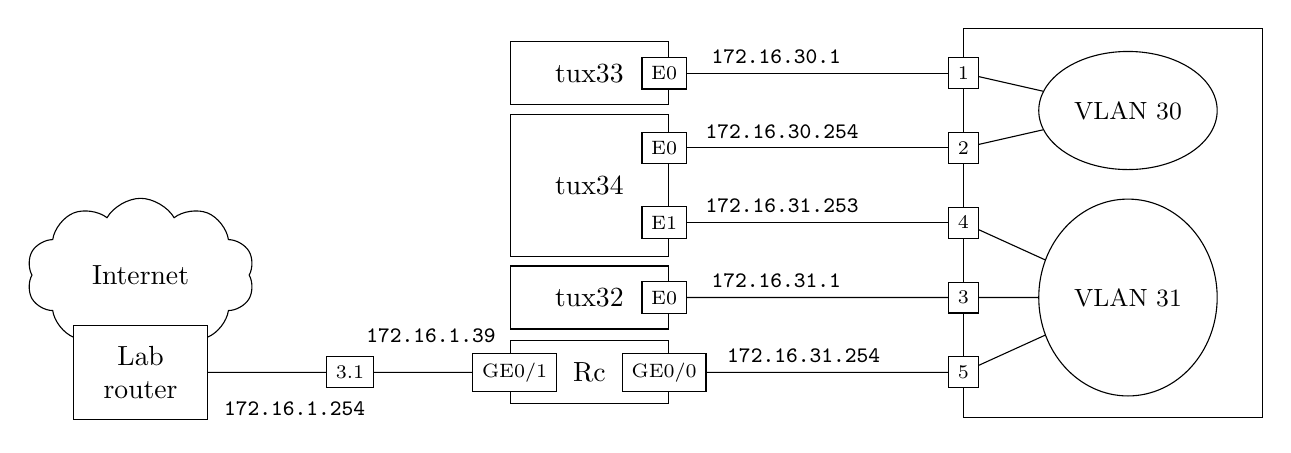
\begin{tikzpicture}[-,>=stealth',node distance=2cm,initial text=$ $,scale=0.95]
        \node at (0,-0) [rectangle,draw,minimum height=0.8cm, minimum width=2cm] (tux33) {tux33};
        \node at (1.0, -0) [rectangle, draw, fill=white] (tux33_E0){ \scriptsize E0 };

        \node at (0,-1.5) [rectangle,draw, minimum height=1.8cm, minimum width=2cm] (tux34) {tux34};
        \node at (1.0, -1) [rectangle, draw, fill=white] (tux34_E0){ \scriptsize E0 };
        \node at (1.0, -2) [rectangle, draw, fill=white] (tux34_E1){ \scriptsize E1 };
        
        \node at (0,-3) [rectangle,draw, minimum height=0.8cm, minimum width=2cm] (tux32) {tux32};
        \node at (1.0, -3) [rectangle, draw, fill=white] (tux32_E0){ \scriptsize E0 };

        \node at (0,-4) [rectangle,draw, minimum height=0.8cm, minimum width=2cm] (Rc) {Rc};
        \node at (1.0, -4) [rectangle, draw, fill=white] (Rc_GE0){ \scriptsize GE0/0 };
        \node at (-1.0, -4) [rectangle, draw, fill=white] (Rc_GE1){ \scriptsize GE0/1 };

        \node at (-3.2, -4) [rectangle, draw, fill=white] (3_1){ \scriptsize 3.1 };

        \node at (-6,-2.7) [cloud, draw,cloud puffs=10,cloud puff arc=120, aspect=1.8, inner ysep=1.2em] {Internet};
        \node at (-6,-4) [rectangle,draw, minimum height=1.2cm, minimum width=1.7cm, align=center, fill=white] (lab_router) {Lab\\router};

        \draw   (5, +0.6) rectangle ++(4, -5.2);
        \node at (7.2, -0.5) [ellipse, draw, minimum height = 1.5cm, minimum width = 2.0cm, align=center] (VLAN30) {\small VLAN 30};
        \node at (7.2, -3.0) [ellipse, draw, minimum height = 2.5cm, minimum width = 2.0cm, align=center] (VLAN31) {\small VLAN 31};
        \node at (5.0, -0.00) [rectangle, draw, fill=white] (switch_1){ \scriptsize 1 };
        \node at (5.0, -1.00) [rectangle, draw, fill=white] (switch_2){ \scriptsize 2 };
        \node at (5.0, -2.00) [rectangle, draw, fill=white] (switch_4){ \scriptsize 4 };
        \node at (5.0, -3.00) [rectangle, draw, fill=white] (switch_3){ \scriptsize 3 };
        \node at (5.0, -4.00) [rectangle, draw, fill=white] (switch_5){ \scriptsize 5 };

        \draw   (tux33_E0)    edge[above, align=left]     node[xshift=-0.45cm]{\footnotesize \texttt{172.16.30.1  }}          (switch_1)
                (tux34_E0)    edge[above, align=left]     node[xshift=-0.45cm]{\footnotesize \texttt{172.16.30.254}}          (switch_2)
                (tux32_E0)    edge[above, align=left]     node[xshift=-0.45cm]{\footnotesize \texttt{172.16.31.1  }}          (switch_3)
                (tux34_E1)    edge[above, align=left]     node[xshift=-0.45cm]{\footnotesize \texttt{172.16.31.253}}          (switch_4)
                (Rc_GE0)      edge[above, align=left]     node[xshift=-0.30cm]{\footnotesize \texttt{172.16.31.254}}          (switch_5)
                (Rc_GE1)      edge[above, align=right]    node[xshift=+0.10cm, yshift=+0.25cm]{\footnotesize \texttt{172.16.1.39}}            (3_1)
                (3_1)         edge[below, align=left]     node[xshift=+0.35cm, yshift=-0.25cm]{\footnotesize \texttt{172.16.1.254}}          (lab_router)

                (switch_1) edge[] (VLAN30)
                (switch_2) edge[] (VLAN30)
                (switch_3) edge[] (VLAN31)
                (switch_4) edge[] (VLAN31)
                (switch_5) edge[] (VLAN31)
            ;

    \end{tikzpicture}
	\caption{Network architecture for experiment 4}
	\label{fig:network_exp4}
\end{figure}

\textbf{Objectives:} configure a commercial router and implement NAT.

\subsubsection{Main configuration commands} \label{sec:Com4}

\begin{center}
    \small
    \begin{tabular}{@{}l | m{67mm} | l@{}}
        {\normalfont\textbf{Dev.}} & {\normalfont\textbf{Description}} & {\normalfont\textbf{Commands}} \\ \hline
        switch & Add port 5 to VLAN31 & \begin{lstlisting}[basicstyle=\linespread{0.85}\ttfamily\small, frame=none, numbers=none, language=cisco]
interface fastethernet 0/5
switchport mode access
switchport access vlan 31
        \end{lstlisting} \\ \hline
        router & Configure interface with VLAN31, set it as the inside of private network & \begin{lstlisting}[basicstyle=\linespread{0.85}\ttfamily\small, frame=none, numbers=none, language=cisco]
interface gigabitethernet 0/0
ip address 172.16.31.254 255.255.255.0
no shutdown
ip nat inside
        \end{lstlisting} \\
        router & Configure interface with lab router, set it as the outside of private network & \begin{lstlisting}[basicstyle=\linespread{0.85}\ttfamily\small, frame=none, numbers=none, language=cisco]
interface gigabitethernet 0/1
ip address 172.16.1.39 255.255.255.0
no shutdown
ip nat outside
        \end{lstlisting} \\
        router & Declare interface with lab router as the sole IP of the new NAT pool & \begin{lstlisting}[basicstyle=\linespread{0.85}\ttfamily\small, frame=none, numbers=none, language=cisco, escapeinside={(*}{*)}]
ip nat pool ovrld
    (*\mbox{\textcolor{red}{$\hookrightarrow$}\space}*)172.16.1.39 172.16.1.39 prefix 24
        \end{lstlisting} \\
        router & Declare the address list 1 can use the NAT pool & \begin{lstlisting}[basicstyle=\linespread{0.85}\ttfamily\small, frame=none, numbers=none, language=cisco, escapeinside={(*}{*)}]
ip nat inside source
    (*\mbox{\textcolor{red}{$\hookrightarrow$}\space}*)list 1 pool ovrld overload
        \end{lstlisting}\\
        router & Allow IP addresses 172.16.30.0-.7 and 172.16.31.0-.7 to use NAT & \begin{lstlisting}[basicstyle=\linespread{0.85}\ttfamily\small, frame=none, numbers=none, language=cisco]
access-list 1 permit 172.16.30.0 0.0.0.7
access-list 1 permit 172.16.31.0 0.0.0.7
        \end{lstlisting}\\
        router & Set lab router as default gateway & \begin{lstlisting}[basicstyle=\linespread{0.85}\ttfamily\small, frame=none, numbers=none, language=cisco]
ip route 0.0.0.0 0.0.0.0 172.16.1.254
        \end{lstlisting}\\
        router & Add route to VLAN30 via tux34 & \begin{lstlisting}[basicstyle=\linespread{0.85}\ttfamily\small, frame=none, numbers=none, language=cisco, escapeinside={(*}{*)}]
ip route 172.16.30.0 255.255.255.0
    (*\mbox{\textcolor{red}{$\hookrightarrow$}\space}*)172.16.31.253
        \end{lstlisting}
    \end{tabular}
\end{center}

\subsubsection{Logs analysis} \label{sec:Log4}

The command \texttt{ip route <dest> <mask> <gw>} is used to configure a static route in a commercial router, where \texttt{<dest>/<mask>} describes the set of IP addresses that can be routed using this rule and \texttt{<gw>} the gateway IP address to route requests to these IP addresses.

\begin{center}
    \begin{tabular}{l | l | l | l | l}
        Redirect & \redcross              & \redcross              & \greencheckmark        & \greencheckmark        \\ \hline
        Route    & \redcross              & \greencheckmark        & \redcross              & \greencheckmark        \\ \hline
        Hop 0    & \texttt{172.16.31.1  } & \texttt{172.16.31.1  } & \texttt{172.16.31.1  } & \texttt{172.16.31.1  } \\
        Hop 1    & \texttt{172.16.31.254} & \texttt{172.16.31.253} & \texttt{\color{gray}172.16.31.254} & \texttt{172.16.31.253} \\
        Hop 2    & \texttt{172.16.31.253} & \texttt{172.16.30.1  } & \texttt{172.16.31.253} & \texttt{172.16.30.1  } \\
        Hop 3    & \texttt{172.16.30.1  } & \texttt{             } & \texttt{172.16.30.1  } & \texttt{             } \\
    \end{tabular}
\end{center}

When running the ping command from tux32 to tux33 without redirects, the packets first arrived on the router and then were redirected to tux34 and after it tux33.

After enabling the redirects and running ping again, the router sends a ICMP redirect message to tux32 that allows tux32 to directly send packets to tux34, without needing to go first through the router.

Network Address Translation (NAT) is a method used by routers for mapping a large private IP address space into usually a single public IP address issued by the ISP to the router \cite{rfc2663}.
NAT has as main advantages to avoid having to issue a worldwide IP address for each interface on the Internet, as well as hide the private network from the rest of the Internet to some extent.
Outbound packets are rewritten to feature the router's public address instead of the device's private address.
The destination of inbound packets is disambiguated using information stored by the router during the outbound phase, thus allowing inbound packets to be rewritten to feature the proper private address.
The most common implementation of NAT is Network Address and Port Translation (NAPT), which disambiguates private IP addresses by mapping each of them to an arbitrary, large port number that is sent in the rewritten outbound packet along with the router's public address; this port number is also featured in the response, thus allowing disambiguation on response reception.

To configure NAT in a commercial router, one should follow the abovementioned configuration commands. Generally speaking, setting up NAT requires one to:
\begin{enumerate*}
    \item Declare the inside and outside interfaces of the private network;
    \item Create a NAT pool from which the router can get a public IP address (usually the pool only has one public IP address);
    \item Declare which private IP addresses can use that NAT pool.
\end{enumerate*}
These steps are to be performed together with other non-NAT-related commands, like setting IP addresses for the router interfaces, creating the required routes to subnets of the private network, and set the default gateway as the interface the router uses to connect to the Internet, which in our case has IP address \texttt{172.16.1.254}. 

\subsection{Experiment 5} \label{sec:Exp5}

\begin{figure}[H]
	\centering
    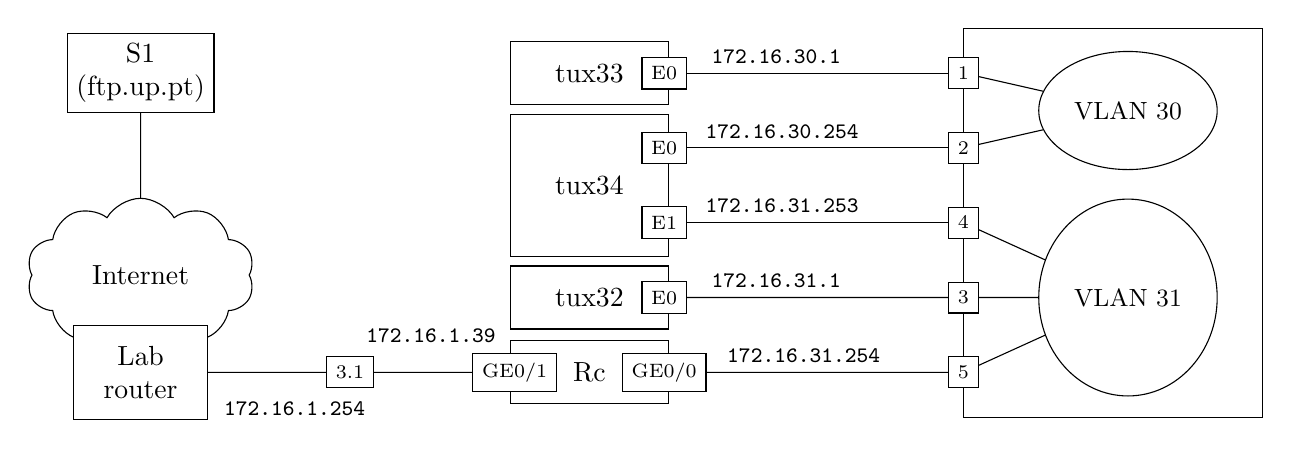
\begin{tikzpicture}[-,>=stealth',node distance=2cm,initial text=$ $,scale=0.95]
        \node at (0,-0) [rectangle,draw,minimum height=0.8cm, minimum width=2cm] (tux33) {tux33};
        \node at (1.0, -0) [rectangle, draw, fill=white] (tux33_E0){ \scriptsize E0 };

        \node at (0,-1.5) [rectangle,draw, minimum height=1.8cm, minimum width=2cm] (tux34) {tux34};
        \node at (1.0, -1) [rectangle, draw, fill=white] (tux34_E0){ \scriptsize E0 };
        \node at (1.0, -2) [rectangle, draw, fill=white] (tux34_E1){ \scriptsize E1 };
        
        \node at (0,-3) [rectangle,draw, minimum height=0.8cm, minimum width=2cm] (tux32) {tux32};
        \node at (1.0, -3) [rectangle, draw, fill=white] (tux32_E0){ \scriptsize E0 };

        \node at (0,-4) [rectangle,draw, minimum height=0.8cm, minimum width=2cm] (Rc) {Rc};
        \node at (1.0, -4) [rectangle, draw, fill=white] (Rc_GE0){ \scriptsize GE0/0 };
        \node at (-1.0, -4) [rectangle, draw, fill=white] (Rc_GE1){ \scriptsize GE0/1 };

        \node at (-3.2, -4) [rectangle, draw, fill=white] (3_1){ \scriptsize 3.1 };

        \node at (-6,-2.7) [cloud, draw,cloud puffs=10,cloud puff arc=120, aspect=1.8, inner ysep=1.2em] (internet) {Internet};
        \node at (-6,-4) [rectangle,draw, minimum height=1.2cm, minimum width=1.7cm, align=center, fill=white] (lab_router) {Lab\\router};

        \node at (-6, -0) [rectangle,draw, minimum height=1.0cm, minimum width=1.7cm, align=center, fill=white] (dns_server) {S1\\(ftp.up.pt)};

        \draw   (5, +0.6) rectangle ++(4, -5.2);
        \node at (7.2, -0.5) [ellipse, draw, minimum height = 1.5cm, minimum width = 2.0cm, align=center] (VLAN30) {\small VLAN 30};
        \node at (7.2, -3.0) [ellipse, draw, minimum height = 2.5cm, minimum width = 2.0cm, align=center] (VLAN31) {\small VLAN 31};
        \node at (5.0, -0.00) [rectangle, draw, fill=white] (switch_1){ \scriptsize 1 };
        \node at (5.0, -1.00) [rectangle, draw, fill=white] (switch_2){ \scriptsize 2 };
        \node at (5.0, -2.00) [rectangle, draw, fill=white] (switch_4){ \scriptsize 4 };
        \node at (5.0, -3.00) [rectangle, draw, fill=white] (switch_3){ \scriptsize 3 };
        \node at (5.0, -4.00) [rectangle, draw, fill=white] (switch_5){ \scriptsize 5 };

        \draw   (tux33_E0)    edge[above, align=left]     node[xshift=-0.45cm]{\footnotesize \texttt{172.16.30.1  }}          (switch_1)
                (tux34_E0)    edge[above, align=left]     node[xshift=-0.45cm]{\footnotesize \texttt{172.16.30.254}}          (switch_2)
                (tux32_E0)    edge[above, align=left]     node[xshift=-0.45cm]{\footnotesize \texttt{172.16.31.1  }}          (switch_3)
                (tux34_E1)    edge[above, align=left]     node[xshift=-0.45cm]{\footnotesize \texttt{172.16.31.253}}          (switch_4)
                (Rc_GE0)      edge[above, align=left]     node[xshift=-0.30cm]{\footnotesize \texttt{172.16.31.254}}          (switch_5)
                (Rc_GE1)      edge[above, align=right]    node[xshift=+0.10cm, yshift=+0.25cm]{\footnotesize \texttt{172.16.1.39}}            (3_1)
                (3_1)         edge[below, align=left]     node[xshift=+0.35cm, yshift=-0.25cm]{\footnotesize \texttt{172.16.1.254}}          (lab_router)

                (switch_1) edge[] (VLAN30)
                (switch_2) edge[] (VLAN30)
                (switch_3) edge[] (VLAN31)
                (switch_4) edge[] (VLAN31)
                (switch_5) edge[] (VLAN31)
                (dns_server) edge[] (internet)
            ;

    \end{tikzpicture}
	\caption{Network architecture for experiment 5}
	\label{fig:network_exp5}
\end{figure}

\textbf{Objectives:} Configure DNS service.

\subsubsection{Main configuration commands} \label{sec:Com5}
\begin{center}
    \small
    \begin{tabular}{@{}m{10mm} | m{39mm} | l@{}}
        {\normalfont\textbf{Dev.}} & {\normalfont\textbf{Description}} & {\normalfont\textbf{Commands}}  \\ \hline
        tux32, tux33, tux34      & Configure DNS & 
        \begin{lstlisting}[frame=none, numbers=none, language=sh, escapeinside={(*}{*)}]]
echo -e "search netlab.fe.up.pt\nnameserver 172.16.1.1"
    (*\mbox{\textcolor{red}{$\hookrightarrow$}\space}*)> /etc/resolv.conf
        \end{lstlisting}
    \end{tabular}
\end{center}
\subsubsection{Logs analysis} \label{sec:Log5}

After tux33 (172.16.30.1) sent a query to the DNS server services.netlab.fe.up.pt (172.16.1.1),
in our logs for www.sapo.pt, 172.16.1.1 sent a query response with the corresponding IP address 213.13.146.142.
This IP address was used afterwards by tux33 to send ICMP packets.

We could also observe a reverse DNS, this is used to identify a domain name with an IP address. 
This was done with a dedicated domain \textit{in-add.arpa}.
Just as DNS domain names are read with the lowest level subdomain occupying the furthest left position and the root at the far right, in-addr.arpa domain IP addresses are read from lowest level to the root. Thus, the IP addresses are read backward \cite{in-addr-arpa}. 
In the logs from wireshark, tux33 sent a query to the DNS Server with 142.146.13.213.in-addr.arpa.
This could be used, for example, by sapo.pt to keep track of traffic origin.

\subsection{Experiment 6} \label{sec:Exp6}

\textbf{Objectives:} Test the download application in the configured network.

\subsubsection{Logs analysis} \label{sec:Log6}

The download application opened two TCP connections. 
The first was used through port 21 to send and receive commands to the server, this connection is responsible for the FTP control information.
The second was opened in the port specified after entering passive mode, this was used to transfer data between the server and the client.

In the first phase of our TCP connection, a connection was stablished with a three-way handshake, a SYN command is sent to the server, the server then replied with a SYN-ACK and the client sent a ACK to the server.
In the second phase happened the data-transfer, where FTP-DATA packets were sent by the server and the client replied with ACK for each successful packet received.
In the third phase, in order to close the connection, the client sent a FIN-ACK, the server replied with FIN-ACK, the client then sent ACK, and the server ended with another ACK. 

The TCP uses the method ARQ (Automatic Repeat Request) to handle errors in the data-transfer.
This method sends ACK (acknowlegdment message) when the data is received successfully before a timeout occurs.
If a timeout does occurs, the data is retransmitted until it is correctly received.

The TCP also have a congestion control mechanism, which uses a congestion window that limits the amount of data this protocol can send into the network, 
so it does not send more than the window size field (specified in bytes) that can be found in the TCP header. 

\begin{figure}
    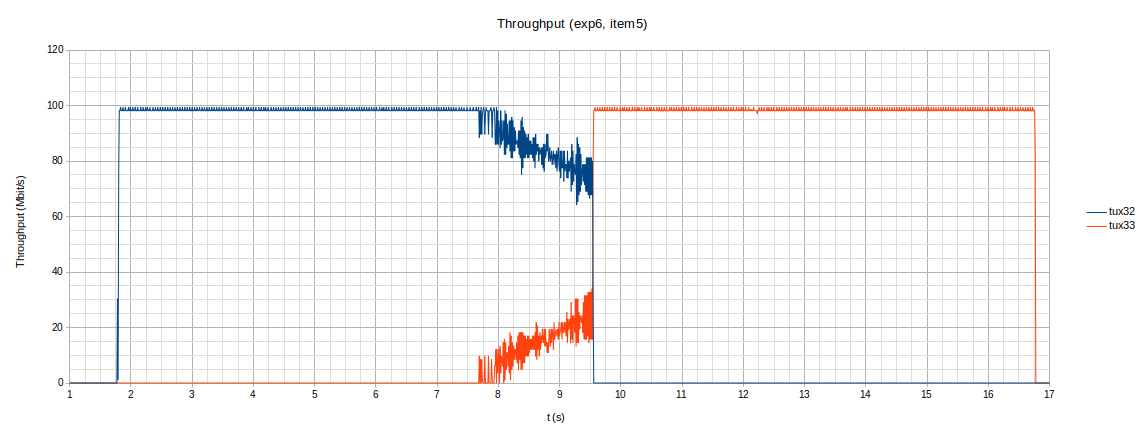
\includegraphics[width=\linewidth]{exp6_item5_hist.png}
    \caption{}
    \label{fig:exp6_item5}
\end{figure}

In this experiment, we tested a simultaneous download in tux32 and tux33. First a download was started at tux32, and some seconds after another download was started at tux33 as seen in \ref{fig:exp6_item5} .
When the second download start we can see the throughput converging and then it quickly rises in tux33 when download in tux32 finishes.

\section*{Conclusion} \label{sec:Conclusion}

This project allowed us to study and configure a network that was used to test a download application.
The results from the download application were successful, being able to connect and establish a data-transfer between FTP servers and the computers from our network. 

Furthermore, we could analyse and discuss the logs from the experiences, which gave us a better understanding of the protocols, methods and the data flow in a network.

\bibliographystyle{acm}
\addcontentsline{toc}{section}{Bibliography}
\bibliography{report}

\appendix
\appendixpage
\addappheadtotoc
\chapter{Source code}

The source code of this project can be obtained from \href{https://github.com/dmfrodrigues/feup-rcom-l2}{github.com/dmfrodrigues/feup-rcom-l2}.
The source code is made available by \textcopyright~Diogo Rodrigues and Breno Pimentel under the \href{https://www.gnu.org/licenses/gpl-3.0.en.html}{GNU General Public License v3} (GPLv3), which you should have received together with the source code, or that you can otherwise obtain online.

During project development and evaluation the repository remained private, although it can be shared with evaluators on request to clarify the development process or due to other justifiable reasons.
It will be made public once all equivalent curricular unit projects have been evaluated in the present school year.

\newgeometry{top=24mm,bottom=24mm,left=14mm,right=14mm}
\fancyhfoffset{0pt}

\lstinputlisting[basicstyle=\ttfamily\small, caption=\texttt{url\_parser.h}, language=C]{../../download/include/url_parser.h}
\lstinputlisting[basicstyle=\ttfamily\small, caption=\texttt{url\_parser.c}, language=C]{../../download/src/url_parser.c}

\lstinputlisting[basicstyle=\ttfamily\small, caption=\texttt{server\_cmds.h}, language=C]{../../download/include/server_cmds.h}
\lstinputlisting[basicstyle=\ttfamily\small, caption=\texttt{server\_cmds.c}, language=C]{../../download/src/server_cmds.c}

\lstinputlisting[basicstyle=\ttfamily\small, caption=\texttt{download.h}, language=C]{../../download/include/download.h}
\lstinputlisting[basicstyle=\ttfamily\small, caption=\texttt{download.c}, language=C]{../../download/src/download.c}

\restoregeometry

\chapter{Configuration commands}
\lstinputlisting[basicstyle=\ttfamily\small, caption=\texttt{tuxy2\_config.sh}, language=bash]{../../part2/config/tuxy2_config.sh}
\lstinputlisting[basicstyle=\ttfamily\small, caption=\texttt{tuxy3\_config.sh}, language=bash]{../../part2/config/tuxy3_config.sh}
\lstinputlisting[basicstyle=\ttfamily\small, caption=\texttt{tuxy4\_config.sh}, language=bash]{../../part2/config/tuxy4_config.sh}
\lstinputlisting[basicstyle=\ttfamily\small, caption=\texttt{switch.sh}, language=cisco]{../../part2/config/switch.sh}
\lstinputlisting[basicstyle=\ttfamily\small, caption=\texttt{router.sh}, language=cisco]{../../part2/config/router.sh}

\newgeometry{top=24mm,bottom=24mm,left=14mm,right=14mm}
\fancyhfoffset{0pt}
\chapter{Logs}

\counterwithin{lstlisting}{subsection}
\renewcommand{\thelstlisting}{%
  \thechapter.\thesubsection(\arabic{lstlisting})%
}

\begin{center}
    \begin{tabular}{l | l | l}
        \textbf{Interface} & \textbf{MAC address}       & \textbf{IP address}    \\ \hline
        tux32-eth0         & \texttt{00:21:5a:61:30:63} & \texttt{172.16.31.1  } \\
        tux33-eth0         & \texttt{00:21:5a:61:24:92} & \texttt{172.16.30.1  } \\
        tux34-eth0         & \texttt{00:21:5a:5a:7d:74} & \texttt{172.16.30.254} \\
        tux34-eth2         & \texttt{00:c0:df:25:26:0a} & \texttt{172.16.31.253} \\
        Rc-GE0/0           & \texttt{68:ef:bd:d6:aa:b8} & \texttt{172.16.31.254} \\
        Rc-GE0/1           & \texttt{                 } & \texttt{172.16.1.39  } \\
    \end{tabular}
\end{center}

\section{Experiment 1}
\setcounter{subsection}{4}
\subsection{Item 5}
\lstinputlisting[basicstyle=\linespread{0.85}\ttfamily\small, frame=tbr, label={1-5-tux33-routes}, caption=\texttt{1-5-tux33-routes.txt}]{../../part2/exp1/1-5-tux33-routes.txt}
\lstinputlisting[basicstyle=\linespread{0.85}\ttfamily\small, frame=tbr, label={1-5-tux33-arp},    caption=\texttt{1-5-tux33-arp.txt}   ]{../../part2/exp1/1-5-tux33-arp.txt}
\lstinputlisting[basicstyle=\linespread{0.85}\ttfamily\small, frame=tbr, label={1-5-tux34-routes}, caption=\texttt{1-5-tux34-routes.txt}]{../../part2/exp1/1-5-tux34-routes.txt}
\lstinputlisting[basicstyle=\linespread{0.85}\ttfamily\small, frame=tbr, label={1-5-tux34-arp},    caption=\texttt{1-5-tux34-arp.txt}   ]{../../part2/exp1/1-5-tux34-arp.txt}

\begin{landscape}
\setcounter{subsection}{9}
\subsection{Item 10}
\lstinputlisting[basicstyle=\linespread{0.85}\ttfamily\scriptsize, frame=tbr, label={listing:1-10-tux33.pcapng}, caption=\texttt{1-10-tux33.pcapng.txt}]{../../part2/exp1/1-10-tux33.pcapng.txt}
\end{landscape}

\begin{landscape}
\section{Experiment 2}

\setcounter{subsection}{4}
\subsection{Item 5}
\lstinputlisting[basicstyle=\linespread{0.85}\ttfamily\scriptsize, frame=tbr, label={listing:2-5-tux33.pcapng}, caption=\texttt{2-5-tux33.pcapng.txt}]{../../part2/exp2/2-5-tux33.pcapng.txt} \pagebreak

\setcounter{subsection}{6}
\subsection{Item 7}

\lstinputlisting[basicstyle=\linespread{0.85}\ttfamily\scriptsize, frame=tbr, label={listing:2-7-tux32.pcapng}, caption=\texttt{2-7-tux32.pcapng.txt}]{../../part2/exp2/2-7-tux32.pcapng.txt} \pagebreak
\lstinputlisting[basicstyle=\linespread{0.85}\ttfamily\scriptsize, frame=tbr, label={listing:2-7-tux33.pcapng}, caption=\texttt{2-7-tux33.pcapng.txt}]{../../part2/exp2/2-7-tux33.pcapng.txt} \pagebreak
\lstinputlisting[basicstyle=\linespread{0.85}\ttfamily\scriptsize, frame=tbr, label={listing:2-7-tux34.pcapng}, caption=\texttt{2-7-tux34.pcapng.txt}]{../../part2/exp2/2-7-tux34.pcapng.txt} \pagebreak

\setcounter{subsection}{9}
\subsection{Item 10}

\lstinputlisting[basicstyle=\linespread{0.85}\ttfamily\scriptsize, frame=tbr, label={listing:2-10-tux32.pcapng}, caption=\texttt{2-10-tux32.pcapng.txt}]{../../part2/exp2/2-10-tux32.pcapng.txt} \pagebreak
\lstinputlisting[basicstyle=\linespread{0.85}\ttfamily\scriptsize, frame=tbr, label={listing:2-10-tux33.pcapng}, caption=\texttt{2-10-tux33.pcapng.txt}]{../../part2/exp2/2-10-tux33.pcapng.txt} \pagebreak
\lstinputlisting[basicstyle=\linespread{0.85}\ttfamily\scriptsize, frame=tbr, label={listing:2-10-tux34.pcapng}, caption=\texttt{2-10-tux34.pcapng.txt}]{../../part2/exp2/2-10-tux34.pcapng.txt}
\end{landscape}

\begin{landscape}
\section{Experiment 3}

\setcounter{subsection}{2}
\subsection{Item 3}
\lstinputlisting[basicstyle=\linespread{0.85}\ttfamily\small, frame=tbr, label={3-7-tux32.route}, caption=\texttt{3-7-tux32.route.txt}]{../../part2/exp3/3-4-tux32.route.txt}
\lstinputlisting[basicstyle=\linespread{0.85}\ttfamily\small, frame=tbr, label={3-7-tux33.route}, caption=\texttt{3-7-tux33.route.txt}]{../../part2/exp3/3-4-tux33.route.txt}
\lstinputlisting[basicstyle=\linespread{0.85}\ttfamily\small, frame=tbr, label={3-7-tux34.route}, caption=\texttt{3-7-tux34.route.txt}]{../../part2/exp3/3-4-tux34.route.txt}

\setcounter{subsection}{6}
\subsection{Item 7}

\lstinputlisting[basicstyle=\linespread{0.85}\ttfamily\scriptsize, frame=tbr, label={3-7-tux33.pcapng}, caption=\texttt{3-7-tux33.pcapng.txt}]{../../part2/exp3/3-7-tux33.pcapng.txt} \pagebreak

\setcounter{subsection}{7}
\subsection{Item 8}

\lstinputlisting[basicstyle=\linespread{0.85}\ttfamily\scriptsize, frame=tbr, label={listing:3-8-tux34-eth0.pcapng}, caption=\texttt{3-8-tux34-eth0.pcapng.txt}]{../../part2/exp3/3-8-tux34-eth0.pcapng.txt} \pagebreak
\lstinputlisting[basicstyle=\linespread{0.85}\ttfamily\scriptsize, frame=tbr, label={listing:3-8-tux34-eth1.pcapng}, caption=\texttt{3-8-tux34-eth1.pcapng.txt}]{../../part2/exp3/3-8-tux34-eth1.pcapng.txt}
\end{landscape}

\begin{landscape}
\section{Experiment 4}

\setcounter{subsection}{2}
\subsection{Item 3}
\lstinputlisting[basicstyle=\linespread{0.85}\ttfamily\scriptsize, frame=tbr, label={4-3-tux33.pcapng}, caption=\texttt{4-3-tux33.pcapng.txt}]{../../part2/exp4/4-3-tux33.pcapng.txt}

\setcounter{subsection}{3}
\subsection{Item 4}
\lstinputlisting[basicstyle=\linespread{0.85}\ttfamily\small     , frame=tbr, label={4-4c-tux32-noredirect-noroute.ping},   caption=\texttt{4-4c-tux32-noredirect-noroute.ping.txt}       ]{../../part2/exp4/4-4c-tux32-noredirect-noroute.ping.txt}
\lstinputlisting[basicstyle=\linespread{0.85}\ttfamily\scriptsize, frame=tbr, label={4-4c-tux32-noredirect-noroute.pcapng}, caption=\texttt{4-4c-tux32-noredirect-noroute.pcapng.txt}     ]{../../part2/exp4/4-4c-tux32-noredirect-noroute.pcapng.txt}
\end{landscape}

\begin{landscape}
\lstinputlisting[basicstyle=\linespread{0.85}\ttfamily\small     , frame=tbr, label={4-4e-tux32-noredirect-noroute.traceroute},  caption=\texttt{4-4e-tux32-noredirect-noroute.traceroute.txt} ]{../../part2/exp4/4-4e-tux32-noredirect-noroute.traceroute.txt}
\lstinputlisting[basicstyle=\linespread{0.85}\ttfamily\small     , frame=tbr, label={4-4f-tux32-noredirect-yesroute.traceroute}, caption=\texttt{4-4f-tux32-noredirect-yesroute.traceroute.txt}]{../../part2/exp4/4-4f-tux32-noredirect-yesroute.traceroute.txt}
\lstinputlisting[basicstyle=\linespread{0.85}\ttfamily\small     , frame=tbr, label={4-4g-tux32-yesredirect-noroute.ping},       caption=\texttt{4-4g-tux32-yesredirect-noroute.ping.txt}      ]{../../part2/exp4/4-4g-tux32-yesredirect-noroute.ping.txt}
\lstinputlisting[basicstyle=\linespread{0.85}\ttfamily\scriptsize, frame=tbr, label={4-4g-tux32-yesredirect-noroute.pcapng},     caption=\texttt{4-4g-tux32-yesredirect-noroute.pcapng.txt}    ]{../../part2/exp4/4-4g-tux32-yesredirect-noroute.pcapng.txt}
\end{landscape}

\begin{landscape}
\setcounter{subsection}{4}
\subsection{Item 5}
\lstinputlisting[basicstyle=\linespread{0.85}\ttfamily\small     , frame=tbr, label={4-5-tux33.ping},   caption=\texttt{4-5-tux33.ping.txt}  ]{../../part2/exp4/4-5-tux33.ping.txt}
\lstinputlisting[basicstyle=\linespread{0.85}\ttfamily\scriptsize, frame=tbr, label={4-5-tux33.pcapng}, caption=\texttt{4-5-tux33.pcapng.txt}]{../../part2/exp4/4-5-tux33.pcapng.txt}
\end{landscape}

\begin{landscape}
\setcounter{subsection}{6}
\subsection{Item 7}
\lstinputlisting[basicstyle=\linespread{0.85}\ttfamily\small     , frame=tbr, label={4-7-tux33.ping},   caption=\texttt{4-7-tux33.ping.txt}  ]{../../part2/exp4/4-7-tux33.ping.txt}
\lstinputlisting[basicstyle=\linespread{0.85}\ttfamily\scriptsize, frame=tbr, label={4-7-tux33.pcapng}, caption=\texttt{4-7-tux33.pcapng.txt}]{../../part2/exp4/4-7-tux33.pcapng.txt}
\end{landscape}

\begin{landscape}
\section{Experiment 5}
\setcounter{subsection}{2}
\subsection{Item 3}
\lstinputlisting[basicstyle=\linespread{0.85}\ttfamily\small     , frame=tbr, label={5-3-tux33.ping},   caption=\texttt{5-3-tux33.ping.txt}  ]{../../part2/exp5/5-3-tux33.ping.txt}
\lstinputlisting[basicstyle=\linespread{0.85}\ttfamily\scriptsize, frame=tbr, label={5-3-tux33.pcapng}, caption=\texttt{5-3-tux33.pcapng.txt}]{../../part2/exp5/5-3-tux33.pcapng.txt}
\end{landscape}

\begin{landscape}
\section{Experiment 6}

\setcounter{subsection}{1}
\subsection{Item 2}
\subsubsection{Transferring \texttt{pipe.txt}}
\lstinputlisting[basicstyle=\linespread{0.85}\ttfamily\small, frame=tbr, label={listing:6-2-tux33-pipe.download}, caption=\texttt{6-2-tux33-pipe.download.txt}]{../../part2/exp6/6-2-tux33-pipe.download.txt}
\lstinputlisting[basicstyle=\linespread{0.85}\ttfamily\tiny , frame=tbr, label={listing:6-2-tux33-pipe.pcapng},   caption=\texttt{6-2-tux33-pipe.pcapng.txt}  ]{../../part2/exp6/6-2-tux33-pipe.pcapng.txt}
\end{landscape}

\begin{landscape}
\subsubsection{Transferring \texttt{pic2.png}}
\lstinputlisting[basicstyle=\linespread{0.85}\ttfamily\small, frame=tbr, label={listing:6-2-tux33-pic2.download}, caption=\texttt{6-2-tux33-pic2.download.txt}]{../../part2/exp6/6-2-tux33-pic2.download.txt}
\lstinputlisting[basicstyle=\linespread{0.85}\ttfamily\tiny , frame=tbr, label={listing:6-2-tux33-pic2.pcapng},   caption=\texttt{6-2-tux33-pic2.pcapng.txt}  ]{../../part2/exp6/6-2-tux33-pic2.pcapng.txt}
\end{landscape}

\begin{landscape}
\setcounter{subsection}{4}
\subsection{Item 5}
\lstinputlisting[basicstyle=\linespread{0.85}\ttfamily\small, frame=tbr, label={listing:6-5-tux32}, caption=\texttt{6-5-tux32.download.txt}]{../../part2/exp6/6-5-tux32.download.txt}
\lstinputlisting[basicstyle=\linespread{0.85}\ttfamily\tiny , frame=tbr,                            caption=\texttt{6-5-tux32.pcapng.txt}  ]{../../part2/exp6/6-5-tux32.pcapng.txt}
\end{landscape}

\begin{landscape}
\lstinputlisting[basicstyle=\linespread{0.85}\ttfamily\small, frame=tbr, label={listing:6-5-tux33}, caption=\texttt{6-5-tux33.download.txt}]{../../part2/exp6/6-5-tux33.download.txt}
\lstinputlisting[basicstyle=\linespread{0.85}\ttfamily\tiny , frame=tbr,                            caption=\texttt{6-5-tux33.pcapng.txt}  ]{../../part2/exp6/6-5-tux33.pcapng.txt}
\end{landscape}

\restoregeometry

\end{document}
